\documentclass[10pt,a4paper]{article}
\usepackage[utf8]{inputenc}
\usepackage[T1]{fontenc}
\usepackage{lmodern}
\usepackage[margin=0.6in]{geometry}
\usepackage{multicol}
\usepackage{graphicx}
\usepackage{xcolor}
\usepackage{titlesec}
\usepackage{fancyhdr}
\usepackage{tikz}
\usepackage{enumitem}
\usepackage{microtype}
\usepackage{tabularx}
\usepackage{booktabs}
\usepackage{hyperref}

% ──── Color Theme ────
\definecolor{primary}{HTML}{1B3A5C}
\definecolor{accent}{HTML}{E74C3C}
\definecolor{secondary}{HTML}{2E86C1}
\definecolor{lightbg}{HTML}{F8F9FA}
\definecolor{darktext}{HTML}{2C3E50}
\definecolor{rulecolor}{HTML}{BDC3C7}

\hypersetup{colorlinks=true,urlcolor=secondary,linkcolor=primary}

% ──── Section Styling ────
\titleformat{\section}{\Large\bfseries\color{primary}}{}{0em}{}[{\color{accent}\titlerule[1.5pt]}]
\titleformat{\subsection}{\large\bfseries\color{secondary}}{}{0em}{}
\titlespacing{\section}{0pt}{14pt}{6pt}
\titlespacing{\subsection}{0pt}{10pt}{4pt}

% ──── Header/Footer ────
\pagestyle{fancy}
\fancyhf{}
\renewcommand{\headrulewidth}{0pt}
\fancyfoot[L]{\small\color{rulecolor}\textit{CS Department Newsletter}}
\fancyfoot[C]{\small\color{rulecolor}\thepage}
\fancyfoot[R]{\small\color{rulecolor}\textit{Spring 2025}}

\setlength{\parindent}{0pt}
\setlength{\parskip}{6pt}
\setlength{\columnsep}{0.8cm}
\setlength{\columnseprule}{0.4pt}
\renewcommand{\columnseprulecolor}{\color{rulecolor}}

\begin{document}

% ════════════════════════════════════════════
% MASTHEAD
% ════════════════════════════════════════════
\begin{tikzpicture}[remember picture, overlay]
  \fill[primary] ([yshift=0cm]current page.north west) rectangle ([yshift=-4.5cm, xshift=\paperwidth]current page.north west);
\end{tikzpicture}

\vspace*{-1.5cm}
\begin{center}
  {\color{white}\fontsize{36}{44}\selectfont\bfseries The Computing Chronicle}\\[6pt]
  {\color{white!80}\large Department of Computer Science --- Stanford University}\\[4pt]
  {\color{accent}\rule{6cm}{2pt}}\\[4pt]
  {\color{white!70}\small Volume 12, Issue 3 \quad|\quad Spring 2025 \quad|\quad Editor: Prof.\\ Maria Santos}
\end{center}

\vspace{0.8cm}

% ════════════════════════════════════════════
% HIGHLIGHTS BAR
% ════════════════════════════════════════════
\colorbox{lightbg}{%
\begin{minipage}{\dimexpr\textwidth-2\fboxsep}
\centering\small\color{darktext}
\textbf{IN THIS ISSUE:}\quad
New AI Research Lab Opening $\bullet$
Faculty Spotlight: Prof.\\ Kim $\bullet$
Student Hackathon Results $\bullet$
Alumni Interview $\bullet$
Upcoming Events
\end{minipage}}

\vspace{0.6cm}

% ════════════════════════════════════════════
% MAIN CONTENT -- Two Columns
% ════════════════════════════════════════════
\begin{multicols}{2}

% ──── Lead Story ────
\section{Department Launches Interdisciplinary AI Research Laboratory}

The Department of Computer Science officially opened the Stanford Interdisciplinary AI Laboratory (SIAL) on March 15, with a ribbon-cutting ceremony attended by university president Dr.\\ Jonathan Blake and industry partners from Google, Microsoft, and NVIDIA.

The \$45 million facility spans 25,000 square feet on the second floor of the newly renovated Gates Building and houses state-of-the-art computing infrastructure, including a cluster of 128 NVIDIA H100 GPUs and dedicated wet lab space for AI-driven biological research.

``This laboratory represents our commitment to developing AI technologies that address humanity's greatest challenges,'' said department chair Prof.\\ Robert Chen at the opening ceremony. ``By bringing together researchers from computer science, medicine, climate science, and the social sciences, we aim to create AI systems that are not only powerful but also responsible and beneficial.''

\textbf{Research Focus Areas:}
\begin{itemize}[leftmargin=1.2em, nosep, itemsep=2pt]
  \item \textbf{AI for Healthcare}: Drug discovery, medical imaging, and personalized medicine
  \item \textbf{Climate AI}: Weather prediction, carbon capture optimization, and sustainable energy
  \item \textbf{Trustworthy AI}: Fairness, interpretability, robustness, and alignment
  \item \textbf{Foundations}: Large language models, multimodal learning, and reasoning
\end{itemize}

The lab will host 12 faculty members, 40 graduate students, and 15 postdoctoral researchers. Industry partnerships include a \$10 million gift from Google DeepMind and a \$5 million equipment grant from NVIDIA.

% ──── Faculty Spotlight ────
\section{Faculty Spotlight: Prof.\\ Soo-Jin Kim}

\subsection{From Seoul to Stanford: A Journey in Computational Biology}

Prof.\\ Soo-Jin Kim joined the department in September 2024 after a distinguished postdoctoral fellowship at the Broad Institute of MIT and Harvard. Her research focuses on developing machine learning methods for understanding gene regulation and predicting the effects of genetic mutations on protein function.

``I was drawn to computer science because of its potential to transform biology,'' Kim said in a recent interview. ``We are generating biological data at an unprecedented rate, and computational methods are essential for making sense of it all.''

Since arriving at Stanford, Kim has already secured a \$1.2 million NIH R01 grant for her project on ``Deep Learning Models for Predicting Variant Effects in Non-Coding Regulatory Regions.'' Her group currently includes three PhD students and two postdocs.

\textbf{Selected recent publications:}
\begin{enumerate}[leftmargin=1.5em, nosep, itemsep=2pt]
  \item Kim, S.-J. et al. ``RegulomeNet: Predicting regulatory variant effects with graph attention networks.'' \textit{Nature Methods}, 2024.
  \item Kim, S.-J. and Park, H. ``Foundation models for genomics: A survey.'' \textit{Nature Reviews Genetics}, 2024.
\end{enumerate}

% ──── Student News ────
\section{Student Hackathon: Record Participation}

The 8th Annual CS Department Hackathon, held over the weekend of February 22--23, drew a record 280 participants organized into 64 teams. This year's theme, ``AI for Social Good,'' challenged students to build applications addressing real-world social challenges in 36 hours.

\subsection{Winning Projects}

\begin{description}[leftmargin=0em, style=nextline, itemsep=4pt]
  \item[1st Place -- ``AccessiVision'' (Team Alpha)]
  A real-time mobile app that uses computer vision to help visually impaired users navigate indoor spaces. The app identifies obstacles, reads signs, and provides audio directions. Built with PyTorch Mobile and ARCore.

  \item[2nd Place -- ``CrisisMap'' (Team Resilience)]
  A platform that aggregates social media posts during natural disasters to create real-time maps of affected areas, resource needs, and safe routes. Uses NLP to classify and geolocate posts.

  \item[3rd Place -- ``FairLend'' (Team Justice)]
  An auditing tool that detects and mitigates bias in lending algorithms. Provides interpretable reports showing how different demographic groups are affected by model decisions.
\end{description}

The winning teams received prizes including internship offers from sponsoring companies and travel grants to present at the ACM Student Research Competition.

\columnbreak

% ──── Alumni Interview ────
\section{Alumni Interview: Dr.\\ Marcus Chen (Ph.D.\\ '18)}

\textit{Dr.\\ Marcus Chen graduated from our department in 2018 and is now VP of Engineering at Anthropic, where he leads the infrastructure team responsible for training large language models.}

\textbf{Q: How did your time at Stanford prepare you for your current role?}

A: The rigorous theoretical foundation I received at Stanford has been invaluable. My work on distributed systems with Prof.\\ Ousterhout taught me how to think about large-scale infrastructure challenges. But equally important were the soft skills---collaborating with researchers from different backgrounds, communicating complex ideas clearly, and managing uncertainty.

\textbf{Q: What advice would you give to current students?}

A: Three things. First, invest in fundamentals---algorithms, systems, and math. Trends come and go, but fundamentals are forever. Second, work on something you genuinely care about; your best work will come from intrinsic motivation. Third, build things. The gap between theory and practice is where the most interesting problems live.

\textbf{Q: What is the most exciting development in AI right now?}

A: I am most excited about AI systems that can reason and plan, not just pattern-match. The progress in chain-of-thought reasoning and tool use suggests we are approaching systems that can genuinely assist with complex intellectual work. But we need to be thoughtful about safety and alignment---these are not afterthoughts but core engineering challenges.

% ──── Upcoming Events ────
\section{Upcoming Events}

\renewcommand{\arraystretch}{1.3}
\begin{tabularx}{\columnwidth}{@{}lX@{}}
\toprule
\textbf{Date} & \textbf{Event} \\
\midrule
Apr 3 & Distinguished Lecture: Prof.\\ Yann LeCun, ``Objective-Driven AI'' \\
Apr 10--11 & Spring Research Symposium \\
Apr 15 & PhD Admissions Visit Day \\
Apr 22 & Industry Panel: ``Careers in AI'' \\
May 1 & Thesis proposal deadline (Fall graduates) \\
May 8 & Department Awards Banquet \\
May 15 & Senior project presentations \\
Jun 15 & Commencement ceremony \\
\bottomrule
\end{tabularx}

% ──── Quick Stats ────
\section{Department by the Numbers}

\begin{center}
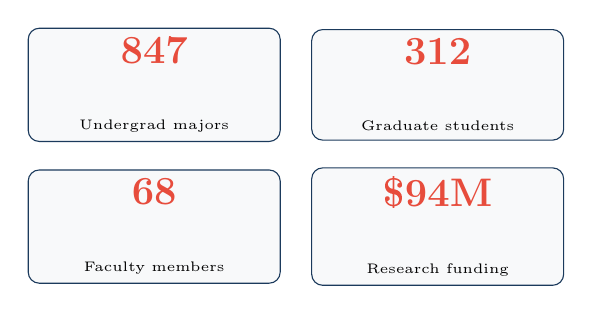
\begin{tikzpicture}[
  statbox/.style={rectangle, draw=primary, fill=lightbg, rounded corners=4pt, minimum width=3.2cm, minimum height=1.4cm, align=center}
]
  \node[statbox] at (0,0) {{\Large\bfseries\color{accent} 847}\\\\{\tiny Undergrad majors}};
  \node[statbox] at (3.6,0) {{\Large\bfseries\color{accent} 312}\\\\{\tiny Graduate students}};
  \node[statbox] at (0,-1.8) {{\Large\bfseries\color{accent} 68}\\\\{\tiny Faculty members}};
  \node[statbox] at (3.6,-1.8) {{\Large\bfseries\color{accent} \$94M}\\\\{\tiny Research funding}};
\end{tikzpicture}
\end{center}

% ──── Announcements ────
\section{Announcements}

\begin{itemize}[leftmargin=1.2em, itemsep=4pt]
  \item \textbf{New course}: CS 329A ``Foundation Models'' will be offered for the first time in Fall 2025, co-taught by Profs.\\ Liang and Hashimoto.
  \item \textbf{Computing resources}: The department cluster has been upgraded with 64 additional A100 GPUs. Submit allocation requests via the department portal.
  \item \textbf{Travel grants}: Applications for the Summer Conference Travel Fund are due May 1. Awards of up to \$2,500 are available.
  \item \textbf{Wellness}: The department peer counseling program holds drop-in hours every Wednesday 3--5pm in Gates 182.
\end{itemize}

\vspace{0.5cm}
\begin{center}
{\color{rulecolor}\rule{0.8\columnwidth}{0.5pt}}\\[6pt]
{\small\color{darktext}
\textbf{The Computing Chronicle} is published quarterly.\\
Submit articles and announcements to \href{mailto:newsletter@cs.stanford.edu}{newsletter@cs.stanford.edu}\\
Back issues: \href{https://cs.stanford.edu/newsletter}{cs.stanford.edu/newsletter}}
\end{center}

\end{multicols}

\end{document}
